%Resume Membuat APlikasi Dengan Flask Swagger

%Kelompok 2 D4 TI / 2B

%Alwan Suryansah				1164033 
%Dinda Ayu Pratiwi				1164034
%Kurnia Sandi					1164042
%Teduh Sanubari					1164054
%Wildan Khaustara Wijaksana		1164058

\documentclass[12pt]{article}
\usepackage{graphicx}    

\begin{document}

\section{Apa itu Flask?}
Flask merupakan microframework yang dibangun dengan
menggunakan bahasa pemrograman Python. Flask digunakan
untuk me-develop sebuah aplikasi web. Flask merupakan
microframework yang artinya flask membuat sebuah pengerjaan
aplikasi web menjadi mudah dan simple karena dapat menjalankan
sebuah web hanya dengan menggunakan 1 file Python. Flask
membuat susunan kerja yang ringan, dan mudah tetapi juga dapat
dikembangkan dengan mudah\cite{gunawan2018aplikasi}.

\section{Apa itu Flask-RESTPlus?}
Flask-RESTPlus bertujuan untuk membuat REST API membangun dengan cepat dan mudah. Ini memberikan cukup gula sintaksis untuk membuat kode Anda mudah dibaca dan mudah dirawat. Fitur pembunuhnya adalah kemampuan untuk secara otomatis menghasilkan dokumentasi interaktif untuk API Anda menggunakan UI Swagger.

\section{Apa itu Swagger?}
Swagger merupakan sebuah open source project dan juga salah satu framework API populer. Swagger dapat digunakan untuk merancang sebuah sistem, membangun sebuah sistem, serta mendokumentasikan dan mengakses API. Dengan adanya swagger, kita bisa melakukan desain ulang atau membuat baru code API dengan editor yang memberikan log jika terjadi error secara real-time.

\section{Sekilas Penjelasan Tentang Membuat Aplikasi dengan Flask Swagger}

\subsection{membuat aplikasi dengan flask dalam jurnal Web Service Dan  Analisis Kinerja Algoritma Klasifikasi Data Mining Untuk Memprediksi Diabetes Mellitus}
membuat aplikasi dengan menggunakan flask web framework, library pandas untuk membaca file csv dan membentuk fitur matrix X dan vektor target y. Penggunan library scikit-learn agar dapat menggunakan modul naive bayes, serta untuk melakukan pembagian data training dan testing dengan fungsi train test split. Modul terakhir yang digunakan adalah pickle untuk menyimpan classifier yang telah dibuat ke dalam disk, agar tidak melakukan training berulang-ulang untuk setiap request yang dikirim \cite{setyawan2017implementasi}. 

\subsection{Reza, Robby and Jati, Agung Nugroho and Ahmad, Umar Ali}
Aplikasi yang dibuat dengan Flask disimpan dalam satu berkas “.py”. Flask adalah framework yang sederhana namun dapat diperluas dengan beragam pustaka tambahan yang disesuaikan dengan kebutuhan penggunanya.membuat aplikasi menggunakan flask akan menjadi sangat cepat, Meskipun Flask belum menyampai versi 1.0 namun dokumentasi yang dmilikinya sangat lengkap\cite{reza2016perancangan}. 

\subsection{Membuat Aplikasi dengan flasgger}
Flasgger adalah salah satu ekstensi Flask yang di gunakan untuk membantu pembuatan API Flask dengan dokumentasi dan live playground yang didukung oleh SwaggerUI. Kemudian Anda juga dapat menentukan struktur API menggunakan file YAML dan Flasgger membuat semuanya sama untuk Anda dan dapat menggunakan skema yang sama untuk memvalidasi sebuah data, Flask dapat membuat susunan kerja yang ringan, dan mudah tetapi juga dapat dikembangkan dengan mudah\cite{gunawan2018aplikasi}.

\subsection{Membuat Aplikasi dengan Flask Menurut Jurnal Aplikasi Pengendali Kamera DSLR Nirkabel Tipe Low End Berbasis Android}
Untuk membuat aplikasi ini terdiri dari tahapan penelitian yang dilakukan. Tahapan tersebut terdiri dari gambaran umum sistem yang akan dijelaskan dalam blok diagram sistem, analisis dan perancangan sistem, analisis dan konfigurasi jaringan yang terdiri dari konfigurasi jaringan berupa konfigurasi interfaces jaringan, konfigurasi IP statis, serta konfigurasi dan pengaturan access point. Tahapan selanjutnya setelah konfigurasi jaringan yaitu tahapan konfigurasi gphoto2 library, konfigurasi ISO, konfigurasi aperture, konfigurasi shutter speed, konfigurasi preview.py, konfigurasi snap.py serta tahapan terakhir yaitu konfigurasi flask API \cite{computingaplikasi}.


\subsection{A Cross-lingual Entity Extraction, Linking and Localization System}
Di bagian ini, kami memperkenalkan API back-end kami.Back-end adalah satu set API RESTful yang dibangun Python Flask, yang merupakan kerangka kerja ringanitu termasuk render template dan hosting serverkemampuan. Kami menggunakan Swagger untuk dokumentasipengelolaan. Selain di-host on-lineAPI, kami juga menerbitkan salinan Docker kami di Dockerhubuntuk distribusi perangkatlunak

Secara umum, kami mengkategorikan API menjadi dua bagian:LARI dan LATIHAN. Bagian RUN bertanggung jawab untuk menjalankan model pra-dilatih untuk 282 bahasa, dan bagian KERETA API menyediakan fungsi pelatihan ulang untuk pengguna yang ingin melatih model pemberian label nama khusus mereka sendiri menggunakan dataset mereka sendiri

Kami juga menerbitkan pelatihan kamidan uji set data, serta sumber daya terkait untuk analisis morfologi dan terjemahan nama di: https://elisa-ie.github.io/wikiann. Meja 1 dan Tabel 2 menyajikan fungsionalitas terperinci dan penggunaan API dari dua bagian ini. Selain komponen inti seperti yang dijelaskan dalam Bagian 2 dan Bagian 3, kami juga menyediakan API komponen tambahan, termasuk yang dapat dilatih ulang komponen transliterasi nama (Lin et al., 2016) dan komponen terjemahan nama dan kata universal berdasarkan alignment kata yang berasal dari salib tautan Wikipedia lingual (Pan et al., 2017). Lebih penggunaan rinci dan contoh dapat ditemukan di kami Dokumentasi Swagger10: https: // elisa-ie. github.io/api 

\begin{figure}[ht]
\centerline{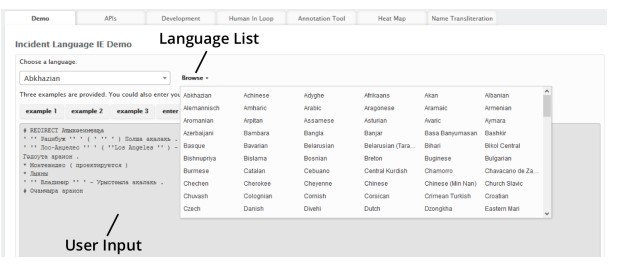
\includegraphics[width=1\textwidth]{satu.JPG}}
\caption{interface uji}
\label{gambarPFS2}
\end{figure}

\begin{figure}[ht]
\centerline{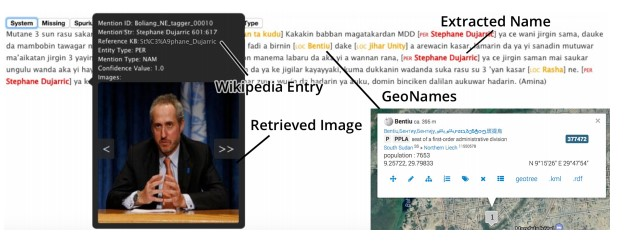
\includegraphics[width=1\textwidth]{dua.JPG}}
\caption{output}
\label{gambarPFS3}
\end{figure}

Gambar 1 menunjukkan antarmuka uji, di mana seorang pengguna dapat memilih salah satu dari 282 bahasa, masukkan teks atau pilih dokumen contoh, dan jalankan sistem. Gambar 2 menunjukkan contoh output. Sebagai tambahan ke ekstraksi entitas dan menghubungkan hasil, kami juga menampilkan 5 gambar teratas untuk setiap entitas yang diambil dari Google Image Search11. Lewat sini bahkan ketika seorang pengguna tidak dapat membaca dokumen dalam sumber rendah bahasa, dia akan mendapatkan tingkat tinggi ringkasan entitas yang terlibat dalam dokumen

memungkinkan untuk dapat melibatkan interface di mana pengguna dapat melihat satu dari banyak bahasa , teks atau pilihan documen , dan dapat di jalankan. dan di dalamnya terdapat output sebagai tambahan ke esktraksi entitas dan menghubungan hasilnya . yang berbentuk bahasa document dalam sumber yang rendah bahasa.\cite{zhangelisa}.

\subsection{membuat aplikasi dengan flask Swagger }
Swagger UI bekerja cukup baik ketika datang untuk menggambarkan dan memvisualisasikan layanan web RESTful. Menghasilkan halaman web kecil yang mendokumentasikan API dan memungkinkan Anda membuat pertanyaan pengujian menggunakan JavaScript (Karzyński, 2016). Keswaggeran didasarkan pada YAML atau JSON, dan merupakan salah satu yang paling populer. The Spesifikasi kompatibel dengan JSON Schema. Muncul dengan alat sumber terbuka untuk menghasilkan dokumentasi dan mensimulasikan server untuk diuji. Namun, antarmuka penggunanya Sepertinya ada banyak ruang untuk perbaikan. Baik klien dan server dihasilkan dan mereka mendokumentasikan secara bersamaan, sehingga mereka diperbarui pada saat yang bersamaan. Pengkodean server terkait erat dengan dokumentasinya, yang memungkinkannya dihasilkan cara yang sangat terintegrasi. Spesifikasi dibuat dari bawah ke atas\cite{ortegacatalogo}.

\subsection{Membuat Aplikasi dengan Flask Swagger}
Dokumentasi Swagger API dibuat secara otomatis dan tersedia di root API Anda tetapi Anda perlu memberikan beberapa detail, Dekorator ini memungkinkan Anda menentukan beberapa detail tentang API Anda, kemudian dapat digunakan dalam deklarasi API Swagger. Dekorator ini berfungsi seperti dekorator Flask-Restful dengan perbedaan yang mendokumentasikan metode. Parameter optionnal memungkinkan Anda untuk menentukan apakah objek dikembalikan sebagai daftar. Anda dapat memberikan dokumentasi kelas-luas dengan menggunakan parameter dokumen Api.route () ‘s’. Ini menerima atribut / sintaks yang sama dari dekorator Api.doc ()\cite{de2017api}.

\subsection{Membuat Aplikasi dengan Flask Swagger}
Flasgger adalah ekstensi Flask untuk membantu pembuatan API Flask dengan dokumentasi dan live playground yang didukung oleh SwaggerUI. Anda dapat menentukan struktur API menggunakan file YAML dan Flasgger membuat semua spesifikasi untuk Anda dan Anda dapat menggunakan skema yang sama untuk memvalidasi data.


\subsection{Membuat Aplikasi dengan Flask Swagger}
Merancang API untuk Layanan ACT dilakukan menggunakan editor Swagger (swagger.io).
Kami merancang lima API untuk memanfaatkan GFE DB: hla, gfe, ars, urutan, dan bertindak. Kita
mendefinisikan parameter dan tanggapan untuk setiap panggilan API dalam kesombongan YAML
spesifikasi. Kami menghasilkan server Python Flask menggunakan file spesifikasi Swagger
dan alat pembuat kode Sombong. Kode server yang dihasilkan telah dimodifikasi untuk diimpor
modul python yang berisi fungsi utama untuk setiap API. Fungsi masing-masing
API dimungkinkan melalui query nol yang mencari GFE DB \cite{halagan2017bioinformatics}

\subsection{Flask Swagger}
Flask-RESTPlus adalah ekstensi untuk Flask yang menambahkan dukungan untuk membangun REST API dengan cepat. Flask-RESTPlus mendorong praktik terbaik dengan penyetelan minimal. Jika Anda terbiasa dengan Flask, Flask-RESTPlus harus mudah diambil. Ini menyediakan koleksi dekorator dan alat untuk mendeskripsikan API Anda dan mengekspos dokumentasi dengan benar (menggunakan Swagger)\cite{buhler2017design}.

\subsection{Membuat Aplikasi dengan Flask Swagger}
Layanan dmon-controller pada dasarnya adalah layanan yang digunakan oleh semua komponen lain untuk berkomunikasi. Ini sebenarnya adalah titik integrasi utama dengan sisa solusi DICE. Secara khusus, ini akan digunakan oleh semua komponen DICE yang membutuhkan data pemantauan. REST API dibagi menjadi dua bagian utama: API Manajemen Pemantauan dan API Kueri Pemantauan \cite{pop2016monitoring}.

\section{Membuat Aplikasi Sederhana Dengan Python Flask + Swagger}

\subsection{Memasang Python}
Apabila komputer kita belum memiliki Python, kita hasrus pasang terlebih dahulu. Apabila, OS komputer/laptop kita tidak memiliki package dari Python, silahkan download di website resmi Python (Recomended Python 3). Jika pengguna OS Windows dengan SWL atau Cygwin,

Untuk memastikan Python telah terpasang dengan baik pada system (Saya menggunakan Windows), buka CMD dan ketikkan python,  Berikut pesan yang seharusnya muncul:

\begin{figure}[ht]
\centerline{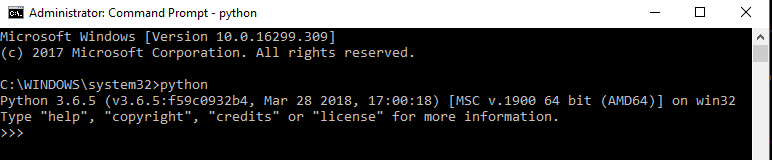
\includegraphics[width=1\textwidth]{5Python.PNG}}
\caption{Python Running}
\label{gambar}
\end{figure}

\subsection{Memasang Flask}
Berikutnya ialah memasang microframework Flask. Tapi, sebelum itu, kami ingin memberitahu kepada anda tentang best practice ketika memasang package Python pada komputer anda.

Dalam Python, package seperti Flask tersedia di repositori publik dimana pengguna dapat mengunduh dan memasangnya. Repositori package resmi Python bernama Python Package Index (PyPI). Ketika menginstall sebuah package dari PyPI akan berjalan cukup mudah karena Python memiliki sebuah tool bernama pip yang dapat melakukan proses pemasangan dengan sendirinya. ntuk memasang package gunakan perintah pip :

\begin{verbatim}
 pip install <package-name>
\end{verbatim}

Python menggunakan konsep virtual environments yang merupakan hasil salinan secara keseluruhan dari interpreter Python. Ketika kita memasang sebuah package di sebuah virtual environment ini maka Python yang berada di sistem utama tidak akan terpengaruh. Virtual environment juga memiliki keuntungan dimana mereka dimiliki oleh user sehingga tidak memerlukan akun administrator.

Mari kita mulai dengan membuat sebuah direktori dimana project kita akan disimpan. Kami akan menamainya microblog karena ini ialah nama aplikasinya:

\begin{verbatim}
C:\WINDOWS\system32>cd/

C:\>mkdir microblog

C:\>cd microblog
\end{verbatim}

Jika menggunakan Python 3, virtual environment sudah ada secara otomatis sehingga bisa langsung dibuat dengan perintah:

\begin{verbatim}
C:\microblog>python3 -m venv venv
\end{verbatim}

Perintah ini mengartikan bahwa kita memerintahkan agar Python menjalankan package venv untuk membuatkan sebuah virtual environment bernama venv. venv pertama di perintah tersebut merupakan nama package-nya sedangkan venv yang kedua merupakan nama direktori untuk menyimpan salinan interpreter Python.


\section{konfigurasi Python Flask + Swagger}
Untuk mengunduh dan memulai aplikasi demo, berikan perintah berikut. Pertama-tama, klon kode aplikasi ke direktori mana pun di disk Anda:
\begin{verbatim}
$ cd /path/to/my/workspace/
$ git clone https://github.com/postrational/rest_api_demo
$ cd rest_api_demo
\end{verbatim}
Buat lingkungan virtual Python dalam direktori bernama venv, aktifkan virtualenv dan pasang dependensi yang diperlukan menggunakan pip:
\begin{verbatim}
$ virtualenv -p `which python3` venv
$ source venv/bin/activate
(venv) $ pip install -r requirements.txt
\end{verbatim}
Sekarang mari siapkan aplikasi untuk pengembangan dan mulai:
\begin{verbatim}
(venv) $ python setup.py develop
(venv) $ python rest_api_demo/app.py
\end{verbatim}
\cite{de2017api}

\subsection{Flask Swagger melalui API}
Saat anda mengakses API melalui UI web Swagger. Hal ini karena tidak mungkin untuk mengatur header otorisasi yang dienkode base64 dari UI angkuh. Bagi mereka yang bertanya-tanya "apa yang angkuh", saya akan mendefinisikan Swagger sebagai alat untuk proyek berbasis API yang menciptakan UI web yang bagus untuk melakukan uji langsung API dan juga mengekspor skema API yang dapat digunakan untuk memahami Definisi API.


\section{Kesimpulan}
dengan dibuatnya resume ini kita dapat mengetahui secara teori tentang pembuatan aplikasi menggunakan bahasa pemrograman pyton yaitu flask + swagger 
\begin{enumerate}
\item mengetahui apa itu flask swagger
\item mengetahui cara pembuatan aplikasi menggunakan flask swagger
\item mengetahui fungsi dari flask swagger itu sendiri
\end{enumerate}	
cukup sekian yang dapat kami sampaikan semoga resume ini dapat bermanfaat  bagi pembaca maupun penulis 

\end{document}
